% fig6-canonical-loop.tex
\documentclass[tikz,border=12pt]{standalone}
% common-styles.tex
% Shared TikZ styles for wonton-proof paper figures

\usepackage{silence}
\WarningFilter{latex}{Missing character} 
\tracinglostchars=0 % Suppress engine-level "Missing character" warnings

\usepackage{fontspec}
\usepackage{unicode-math}

% Use filenames for reliability with Tectonic
\setmainfont{LibertinusSerif-Regular.otf}[
    BoldFont=LibertinusSerif-Bold.otf,
    ItalicFont=LibertinusSerif-Italic.otf,
    BoldItalicFont=LibertinusSerif-BoldItalic.otf
]
\setsansfont{LibertinusSans-Regular.otf}[
    BoldFont=LibertinusSans-Bold.otf,
    ItalicFont=LibertinusSans-Italic.otf
]
\setmonofont{LibertinusMono-Regular.otf}

% Try a more standard math font if LibertinusMath is causing nullfont issues
\setmathfont{LibertinusMath-Regular.otf}
% \setmathfont{latinmodern-math.otf}[range=digits] 

\usepackage{amsmath}
\usepackage{tikz}
\usepackage{forest}

\usetikzlibrary{
    arrows.meta,
    calc,
    decorations.pathreplacing,
    fit,
    positioning,
    shapes.geometric,
    shapes.misc,
    backgrounds,
    shadows.blur,
    fadings
}

% Color palette (muted, print-friendly)
\definecolor{ink}{RGB}{45,45,52}
\definecolor{muted}{RGB}{115,115,125}
\definecolor{highlight}{RGB}{198,120,44}
\definecolor{accentblue}{RGB}{86,130,178}
\definecolor{accentgreen}{RGB}{84,156,132}
\definecolor{blocked}{RGB}{140,75,75}
\definecolor{goalnode}{RGB}{255,255,255}
\definecolor{terminal}{RGB}{238,239,244}
\definecolor{deadnode}{RGB}{248,245,245}
\definecolor{flowbox}{RGB}{250,250,252}
\definecolor{basin1}{RGB}{224,234,248}
\definecolor{basin2}{RGB}{246,232,221}
\definecolor{basin3}{RGB}{228,242,234}
\definecolor{heatbase}{RGB}{86,130,178}

\tikzset{
    line cap=round,
    line join=round,
    pop/.style={
        blur shadow={shadow blur steps=5, shadow blur extra rounding=1.3pt}
    },
    base node/.style={
        rounded rectangle,
        draw=ink,
        line width=0.6pt,
        fill=goalnode,
        text=ink,
        minimum width=2.2cm,
        minimum height=0.7cm,
        align=center,
        pop
    },
    goal/.style={base node, fill=goalnode},
    terminal/.style={base node, fill=terminal, line width=0.9pt},
    dead/.style={base node, fill=deadnode, dashed},
    flowbox/.style={
        rectangle,
        draw=muted,
        rounded corners=3pt,
        fill=flowbox,
        minimum width=1.8cm,
        minimum height=0.6cm,
        align=center,
        font=\normalfont\small,
        text=ink,
        pop
    },
    decision/.style={
        diamond,
        draw=muted,
        fill=flowbox,
        aspect=2.4,
        font=\normalfont\small,
        inner sep=1pt,
        text=ink
    },
    protocolbox/.style={
        rectangle,
        draw=muted,
        rounded corners=4pt,
        fill=flowbox,
        minimum width=2cm,
        minimum height=0.8cm,
        font=\normalfont\small,
        align=center,
        text=ink
    },
    tactic/.style={
        ->,
        >=Stealth,
        draw=muted,
        line width=0.75pt
    },
    tacticlight/.style={
        ->,
        >=Stealth,
        draw=muted!45,
        dashed,
        line width=0.6pt
    },
    backprop/.style={
        ->,
        >=Stealth,
        draw=muted!70,
        dashed,
        line width=0.6pt
    },
    selected/.style={
        tactic,
        draw=highlight,
        line width=1.4pt
    },
    divergetactic/.style={
        tactic,
        draw=highlight,
        line width=1.4pt
    },
    divergenode/.style={
        base node,
        draw=highlight,
        line width=1.0pt
    },
    divergeblock/.style={
        blockedtactic,
        line width=1.2pt
    },
    blockedtactic/.style={
        tactic,
        draw=blocked,
        densely dashed
    },
    flowarrow/.style={
        ->,
        >=Stealth,
        draw=muted,
        line width=0.75pt
    },
    crosslink/.style={
        -,
        draw=muted!70,
        dotted,
        line width=0.6pt
    },
    annot/.style={
        font=\normalfont\footnotesize,
        text=muted
    },
    visit/.style={
        annot,
        font=\normalfont\scriptsize
    },
    annotbg/.style={
        annot,
        fill=white,
        inner sep=1.5pt
    },
    tacticlabel/.style={
        annot,
        font=\ttfamily\footnotesize,
        text=muted
    },
    formula/.style={
        font=\normalfont\footnotesize,
        draw=muted,
        rounded corners=2pt,
        fill=white,
        inner sep=3pt
    },
    paneltitle/.style={
        font=\normalfont\bfseries,
        text=ink
    },
    trajectory/.style={
        ->,
        draw=muted!70,
        line width=0.6pt
    }
}

\begin{document}
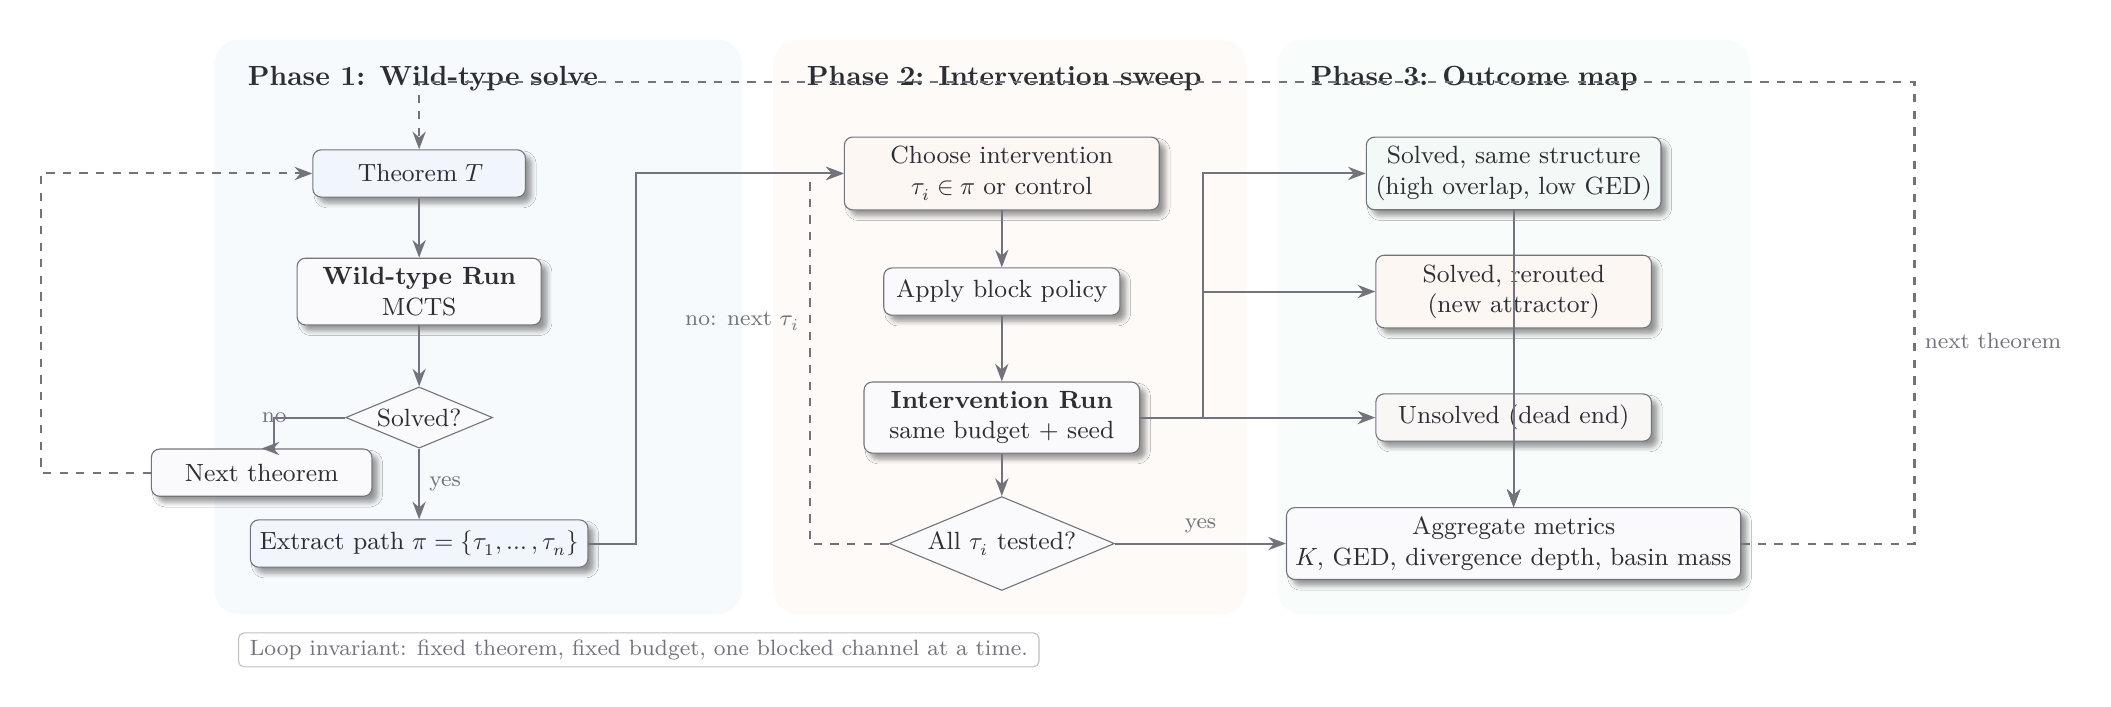
\begin{tikzpicture}[
    node distance=1.6cm and 2.2cm,
    every node/.style={font=\small},
    show background rectangle,
    background rectangle/.style={fill=white}
]

% Phase backgrounds
\path[fill=basin1!25, rounded corners=9pt] (-9.5, 2.5) rectangle (-2.8, -4.8);
\path[fill=basin2!20, rounded corners=9pt] (-2.4, 2.5) rectangle (3.6, -4.8);
\path[fill=basin3!25, rounded corners=9pt] (4.0, 2.5) rectangle (10.0, -4.8);

% Headers
\node[paneltitle, anchor=west] at (-9.2, 2.0) {Phase 1: Wild-type solve};
\node[paneltitle, anchor=west] at (-2.1, 2.0) {Phase 2: Intervention sweep};
\node[paneltitle, anchor=west] at (4.3, 2.0) {Phase 3: Outcome map};

% Left phase
\node[flowbox, fill=basin1!45, minimum width=2.7cm] (thm) at (-6.9, 0.8) {Theorem $T$};
\node[flowbox, minimum width=3.1cm] (wild) at (-6.9, -0.7) {\textbf{Wild-type Run}\\MCTS};
\node[decision] (solved) at (-6.9, -2.3) {Solved?};
\node[flowbox, fill=basin1!45, minimum width=3.8cm] (path) at (-6.9, -3.9) {Extract path $\pi=\{\tau_1,\dots,\tau_n\}$};
\node[flowbox, minimum width=2.8cm] (next1) at (-8.9, -3.0) {Next theorem};

\draw[flowarrow] (thm) -- (wild);
\draw[flowarrow] (wild) -- (solved);
\draw[flowarrow] (solved) -- node[midway, right, annot] {yes} (path);
\draw[flowarrow] (solved.west) -- ++(-0.9,0) |- node[pos=0.25, above, annot] {no} (next1.north);

% Middle phase
\node[flowbox, fill=basin2!35, minimum width=4.0cm] (pick) at (0.5, 0.8) {Choose intervention \\ $\tau_i \in \pi$ or control};
\node[flowbox, minimum width=3.0cm] (apply) at (0.5, -0.7) {Apply block policy};
\node[flowbox, minimum width=3.5cm] (rerun) at (0.5, -2.3) {\textbf{Intervention Run}\\same budget + seed};
\node[decision] (doneall) at (0.5, -3.9) {All $\tau_i$ tested?};

\draw[flowarrow] (path.east) -- ++(0.6,0) |- (pick.west);
\draw[flowarrow] (pick) -- (apply);
\draw[flowarrow] (apply) -- (rerun);
\draw[flowarrow] (rerun) -- (doneall);
\draw[flowarrow, dashed] (doneall.west) -- ++(-1.0,0) |- node[pos=0.3, left, annot] {no: next $\tau_i$} (pick.west);

% Right phase outcomes
\node[flowbox, fill=basin3!45, minimum width=3.5cm] (same) at (7.0, 0.8) {Solved, same structure\\(high overlap, low GED)};
\node[flowbox, fill=basin2!35, minimum width=3.5cm] (alt) at (7.0, -0.7) {Solved, rerouted\\(new attractor)};
\node[flowbox, fill=deadnode!85, minimum width=3.5cm] (fail) at (7.0, -2.3) {Unsolved (dead end)};
\node[flowbox, minimum width=4.4cm] (metrics) at (7.0, -3.9) {Aggregate metrics\\$K$, GED, divergence depth, basin mass};

\draw[flowarrow] (rerun.east) -- ++(0.8,0) |- (same.west);
\draw[flowarrow] (rerun.east) -- ++(0.8,0) |- (alt.west);
\draw[flowarrow] (rerun.east) -- ++(0.8,0) |- (fail.west);
\draw[flowarrow] (same) -- (metrics);
\draw[flowarrow] (alt) -- (metrics);
\draw[flowarrow] (fail) -- (metrics);
\draw[flowarrow] (doneall) -- node[midway, above, annot] {yes} (metrics);
\draw[flowarrow, dashed] (next1.west) -- ++(-1.4,0) |- (thm.west);
\draw[flowarrow, dashed] (metrics.east) -- ++(2.2,0) |- node[pos=0.22, right, annot] {next theorem} ([yshift=0.85cm]thm.north) -- (thm.north);
\node[
    annotbg,
    draw=muted!45,
    rounded corners=2pt,
    anchor=west,
    inner xsep=4pt,
    inner ysep=2.5pt
] at (-9.2, -5.25) {Loop invariant: fixed theorem, fixed budget, one blocked channel at a time.};

\end{tikzpicture}
\end{document}
